\documentclass[11pt]{article}
\usepackage[utf8]{inputenc}
\usepackage[margin=1in]{geometry}

\usepackage{algorithm}
\usepackage[noend]{algpseudocode}
\algnewcommand\algorithmicforeach{\textbf{for each}}
\algdef{S}[FOR]{ForEach}[1]{\algorithmicforeach\ #1\ \algorithmicdo}
\algnewcommand\Not{\textbf{not}\ }

\title{Minimum Spanning Trees}
\author{Larry Wang and Charles Zhao}
\date{October 3, 2016}

\usepackage{tikz}

\usetikzlibrary{calc,shapes.multipart,chains,arrows,positioning}

\tikzstyle{vertex}=[draw,fill=myseagreen,circle,minimum size=24pt,inner sep=0pt]

\definecolor{myseagreen}{RGB}{220,220,220}

\begin{document}

\maketitle

\section{Introduction}
A \textit{spanning tree} of a connected, undirected, and weighted graph $G$ is a subgraph that is a tree including all the vertices of $G$. The Minimum Spanning Tree (MST) problem is the problem of finding a spanning tree of $G$ with minimal total edge weight. Note that if not all edge weights are distinct, then there may be multiple MSTs for a given graph.

\begin{center}
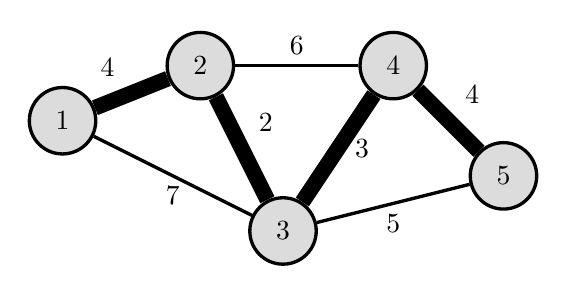
\begin{tikzpicture}[very thick,edge from parent/.style={draw,<-},level/.style={sibling distance=30mm/#1},scale=0.7]
\draw (0, 1) node [vertex] (v1) {1};
\draw (2.5, 2) node [vertex] (v2) {2};
\draw (4, -1) node [vertex] (v3) {3};
\draw (6, 2) node [vertex] (v4) {4};
\draw (8, 0) node [vertex] (v5) {5};
\draw[line width=2mm] (v1) -- (v2) node[midway, above left] {4};
\draw[line width=2mm] (v2) -- (v3) node[midway, above right] {2};
\draw (v1) -- (v3) node[midway, below] {7};
\draw (v2) -- (v4) node[midway, above] {6};
\draw[line width=2mm] (v3) -- (v4) node[midway, right] {3};
\draw (v3) -- (v5) node[midway, below] {5};
\draw[line width=2mm] (v4) -- (v5) node[midway, above right] {4};
\end{tikzpicture}
\end{center}

\section{Kruskal's Algorithm}

Kruskal's Algorithm finds the MST by greedily adding edges; for all edges not yet in the MST, we can repeatedly add the edge of minimum weight to the MST except when adding said edge forms a cycle (which violates the tree structure). This can be done by sorting the edges in order of non-decreasing weight. Furthermore, we can easily determine whether adding an edge will create a cycle in (for all practical purposes) constant time using Union Find. Note that since the most expensive operation is sorting the edges, the computational complexity of Kruskal's Algorithm is $O(E \log E)$. 

To see why this will always work, assume that we are trying to add edge $e$, which connects vertices $u$ and $v$, to the MST. If the only path between $u$ and $v$ is through $e$, then adding $e$ cannot form a cycle, and Kruskal will add $e$ to the MST. However, assume that another path from $u$ to $v$ exists. This path consists of a sequence of edges. By Kruskal, any of these edges with weight less than $e$ are already in the MST. If all of these edges have weight less than the weight of $e$, then we skip over $e$ since adding it would create a cycle. Otherwise, note that $e$ has a lower weight than any of the edges in this path that are not yet in the MST, so adding $e$ is optimal.

\begin{algorithm}[H]
\caption{Kruskal's Algorithm}
\begin{algorithmic}
    \Function{Kruskal}{$v$, $e$}
        \State $e \gets \Call{Sort}{e}$
        \State UnionFind $uf \gets \Call{UnionFind}{v}$
        \ForEach{$edge \in e$}
            \If {$\Not \Call{SameSet}{edge.first, edge.second}$}
                \State $\Call{Union}{edge.first, edge.second}$
            \EndIf
        \EndFor
        \State \Return $uf[0]$
    \EndFunction
\end{algorithmic}
\end{algorithm}

\section{Prim's Algorithm}

Rather than greedily adding edges, Prim's algorithm greedily adds vertices; on each iteration, we add the vertex that is closest to the current MST until all vertices have been added. The process of finding the closest vertex to the MST can be done efficiently using a priority queue in $O(\log N)$. After removing a vertex, we add all of its neighbors that are not yet in the MST to the priority queue and repeat. To begin the algorithm, we simply add any vertex to the priority queue. Note that Prim's algorithm has complexity $O(E \log E)$ since in the worst case every edge will be checked and its corresponding vertex will be added to the priority queue. However, this can be improved to $O(E \log V)$ if we were to update the distances of vertices in the priority queue rather than re-add them. This keeps the maximum size of the priority queue bounded at $V$. Note that this optimization usually isn't necessary for competitive programming. 

Alternatively, we may linearly search for the closest vertex instead of using a priority queue. Each linear pass runs in time $O(V)$, and this must be repeated $V$ times. Thus, this version of Prim's algorithm has complexity $O(V^2)$. Note that this complexity is preferable for dense graphs (in which $E \approx V^2$). 

To see why Prim's algorithm works, consider a cut of the graph partitioning the graph into two sets of vertices $A$ and $B$. Now consider the set of edges $E$ connecting a vertex in $A$ to a vertex in $B$. Note that at least one edge in $E$ must be in the MST. This means that the edge in $E$ with minimum weight must be in the MST. To prove Prim's Algorithm, make $A$ the set of vertices currently in the MST and $B$ the set of all other vertices. Adding the vertex closest to the current MST is equivalent to adding the edge of minimum weight between $A$ and $B$. Prim's Algorithm follows by repeating this process.\footnote {\label{note1}pseudocode taken from Sam Hsiang's \textit{Crash Course Coding Companion}}

\begin{algorithm}[H]
\caption{Prim}
\begin{algorithmic}
\ForAll{vertices $v$}
	\State $dist(v) \gets \infty$
	\State $visited(v) \gets 0$
    \State $prev(v) \gets -1$
\EndFor
\State $dist(src) \gets 0$
\While{$\exists v$ s.t. $visited(v)=0$}
	\State $v \equiv v$ s.t. $visited(v)=0$ with min $dist(v)$
    \State $visited(v) \gets 1$
	\ForAll{neighbors $u$ of $v$}
    	\If{$visited(u) = 0$}
			\If{$weight(v, u) < dist(u)$}
				\State $dist(u) \gets weight(v, u)$
   	        	\State $prev(u) \gets v$
			\EndIf
        \EndIf
    \EndFor
\EndWhile
\end{algorithmic}
\end{algorithm}

\section{Problem Variants}

\subsection{Minimum Spanning Subgraph}

What do you do if some of the edges are already fixed? It doesn't matter if the fixed edges form a cycle, simply continue running Kruskal's algorithm on the remaining edges.

\subsection{Minimax and Maximin}

The minimax problem is the problem of finding a path between two vertices such that the maximum edge weight is minimal. Since this problem wants a path with low individual edge weights regardless of the length (i.e. number of edges) of the path, using an MST is a good idea. The solution to the minimax problem is the maximum edge weight along the path between the two vertices in the MST. 

Analogously, the maximin problem is to find a path between two vertices such that the minimum edge weight is maximal. The solution to the maximin problem is very similar, except we use a maximum spanning tree instead. The maximum spanning tree can be found by finding the MST of the graph where all of the edge weights are negated. 

\section{Problems}

\begin{enumerate}
    \item USACO February 2015 Contest, Silver Problem 3. Superbull
    \item USACO February 2016 Contest, Platinum Problem 2. Fenced In
\end{enumerate}

\end{document}
